\documentclass[10pt,twocolumn,letterpaper]{article}
\usepackage{cvpr}
\usepackage[hyphens]{url}
\usepackage{times}
\usepackage{graphicx}
\usepackage{amsmath}
\usepackage{amssymb}
\usepackage[pagebackref=true,breaklinks=true,colorlinks,bookmarks=false]{hyperref}
\def\GroupID{G01} % <------- ENTER YOUR COMP 6321 group number here

\begin{document}
\title{Fake or Real News? A Comparison of Traditional Machine Learning Models and Deep Learning Models for News Article Classification}
\author{Giselle Martel ID: 26352936 \and Firas Sawan ID: 26487815}
\maketitle

\begin{abstract}
   "Fake news" is a term which we hear more often in contemporary times, and "is part of a larger spectrum ranging from unintentional misinformation (e.g., sloppy reporting) to intentional disinformation (e.g., propaganda)"\cite{doi:https://doi.org/10.1002/9781118841570.iejs0128}. The spread of falsehoods and inaccuracies through social media and online news sources undermines societal progress, and can spawn a multitude of negative effects [CITE]. Thus, the objective of our project is explore the feasibility and performance of existing supervised machine learning and natural language processing techniques in the identification of "fake news" to explore solutions that address misinformation in the digital age. We compare binary classification performance of news articles into "fake" or "real" categories by training six different machine learning models. Traditional classifiers such as Logistic Regression, Decision Tree, Random Forest, Support Vector Machines, and Multinomial Naive Bayes classification were utilized in our experiments, in addition to a Convolutional Neural Network. The results show that Logistic regression has the highest level of accuracy and lowest level of overfitting, thus it was generally the best model to use for classifying articles into the two categories. This classifier was followed in terms of accuracy and performance by the other 4 classifiers in the order mentioned above and the results are presented in the following report. 
\end{abstract} 

%------------------------------------------------------------------------
\section{Introduction}
\textcolor{blue}{State your goal by giving give an example of the data you're working with and an example of the kind of prediction you hope to achieve. Don't bother with a literature review of your subject area, but do mention any important sources you directly relied upon.}\\

The term “fake news” mainly refers to false or inaccurate information that is mistakenly or inadvertently created or spread. Such information is often presented in the form of reputable news, despite the often omission of verifiable facts or sources, deliberately inflammatory language, and the presentation of an issue from one polarized viewpoint [CITATION NEEDED]. In regards to the current COVID-19 global health crisis we are facing, and the recent 2020 U.S. elections, we have witnessed as a society the exponential spread of conspiracies, accusations, and falsehoods which is often fueled by misleading or suspicious sources [CITATION NEEDED]. Such a situation can have a multitude of negative outcomes and undermines progress in several areas of society ranging from politics, health, economics, social justice, and beyond [CITATION NEEDED]. 

Given our concern with this issue, the purpose of our project is to explore machine learning models that can aid in the identification of misleading or untruthful news articles online. We would like to identify, if any, existing popular machine learning models that could accurately classify online new sources by text into "fake" and "real" labels. We will compare the the pros and cons of five different traditional supervised models in text classification; which include Logistic Regression, Decision Tree, Random Forest, Support Vector Machine, and Multinomial Naive Bayes classifiers. In addition, we will compare the results with a supervised deep Convolutional Neural Network. Hyper-parameter tuning will be employed for all models in an attempt to generate a successful result.

To train our collection of models, we utilized an existing dataset from Kaggle of news articles collected between 2015-2018 [CITE], in addition to data which was collected via scraping of more recent articles from both trusted and illegitimate news sources. The following scraped sources were included and labelled as "real" news: CBC news, CTV news, Global news, The Guardian, Fox News, NBC, The Washington Post, BBC, and CNN which are all generally recognized as reputable. More questionable scraped sources such as Breitbart, Infowars, Prntly, National Report, and Daily Buzz Live were labelled as "fake" and included in the dataset. In addition, well-know satirical news sources such as "The Onion" and "The Beaverton" were also included in the data and labelled as "fake".  The top figure below depicts the structure of the dataset from Kaggle, and the bottom figure shows the scraped data before preprocessing:

\begin{center}
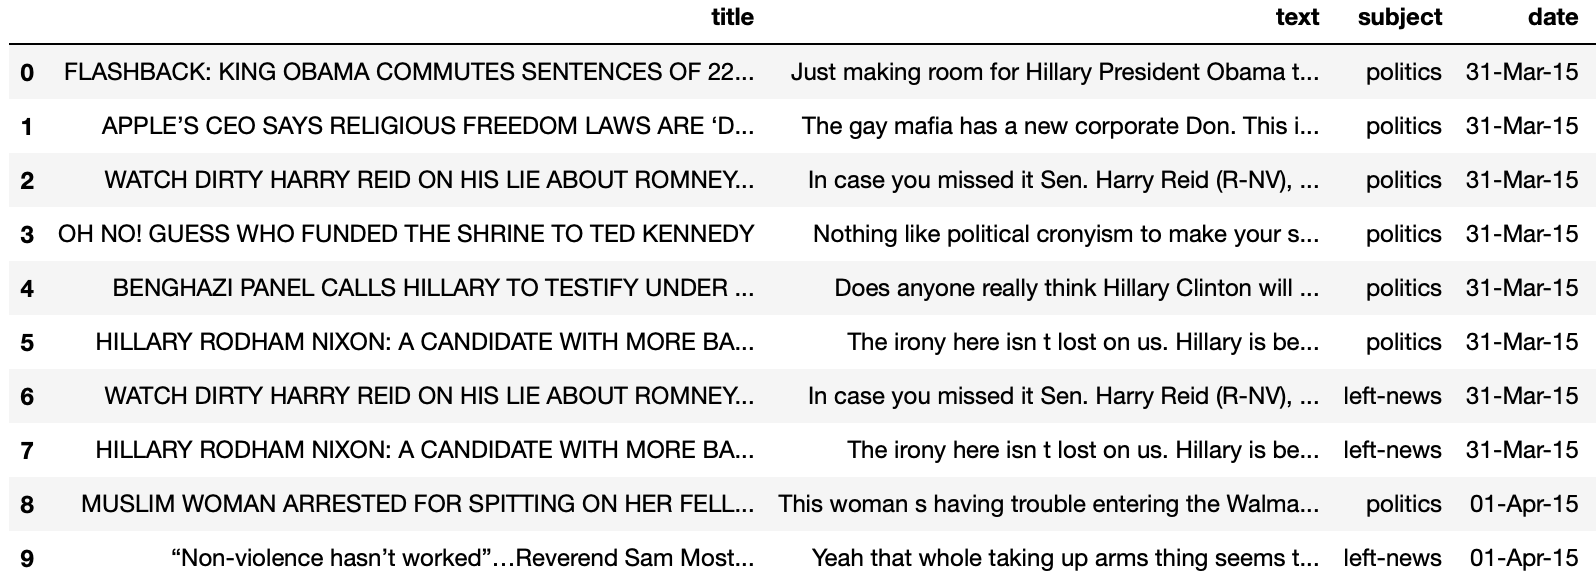
\includegraphics[width=\linewidth]{Latex_Report/report/Graphs/dt_example.png}
\end{center}

\begin{center}
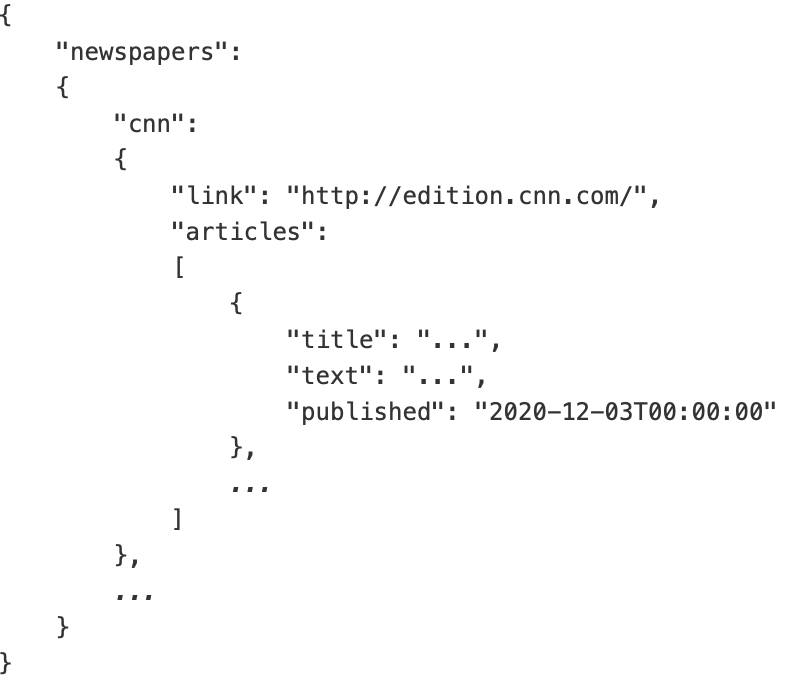
\includegraphics[width=\linewidth]{Latex_Report/report/Graphs/scraped_example.png}
\end{center}

Our inspiration to utilize the Kaggle dataset in addition to a scraping approach came from a similar experiment in news classification conducted by Ria Gandhi [CITATION HERE]. In addition, her approach in preprocessing of the data and her model selection were somewhat replicated in our project, albeit with many changes to implementation details and parameter tuning. The underlying goal of this experiment is to present the respective results from each model and compare their overall performance in classification. The results of our model training and the generated predictions will be presented analyzed in this report. Detailed graphs, confusion matrices, metrics measurement, and other results  for each of the classifiers as well as a report of accuracy, precision and recall metrics. 


%------------------------------------------------------------------------
\section{Methodology \& Experimental Results}

\textcolor{blue}{Describe the important steps you took to achieve your goal, alongside experimental results that followed. If certain steps (preprocessing, extra features, etc.) turned out to be important for maximizing prediction performance, then try to mention how much benefit you observed with/without that feature.}

The first step we had to take to prepare for our experiment was to preprocess our data. This was an important step given that we needed maximize prediction performance by getting rid of empty data cells as well as formatting all entries in each column of both datasets in a similar manner. Preprocessing the data involved parsing both datasets, clearing out empty data cells and formatting the date columns in a uniform manner for all cells. It also involved assigning each dataset their respective labels of fake vs true news. Once this was done, both files were joined together to create one big dataset that we later used in our tokenization process. Tokenization was a necessary process that allowed us to extract all unique words from the joined dataset while excluding some stop-words that were present in abundance throughout the data. Following tokenization the data was split into training and testing components. We opted to split the data into a 70\% training set and a 30\% testing set as it seemed ideal to have our training data consisting of more than double that of the testing data. Following the split we generated a score graph, a document-term matrix for each of the training and testing data and converted both the testing and training datasets into dataframes that we later used in our models. \\

The first model we worked on was the Logistic Regression classifier that we used to predict the probability of our categorically dependent tokenized text. We used the corresponding Sklearn library to generate our model and fit our data to it using hyper parameters obtained via a hyper parameter search for values of C with the help of GridSearchCV method. The search allowed us to obtain the best possible accuracy, calculate the training and testing scores as well as to determine overfitting and perform prediction calculations. The model worked in such a way that it treated our tokenized data as binary variables that contain data coded as 1 (in our case Real) or 0 (in our case "fake") and used this data to make predictions. We subsequently generated a graph of each of the training and testing scores as well as a confusion matrix (Figure~\ref{first_figure}) that helped us visualize the result. The model successfully achieved an accuracy of 91.34\%, a mean squared error of 9.62\% and a precision of 90.78\% with a very low overfitting value of 0.009. \\

\begin{figure}[h]
   \begin{center}
        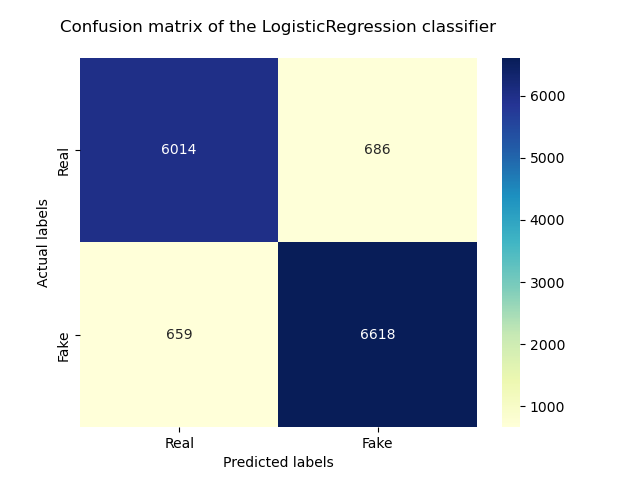
\includegraphics[width=\linewidth]{Latex_Report/report/Graphs/LR/confusion_matrix.png}
        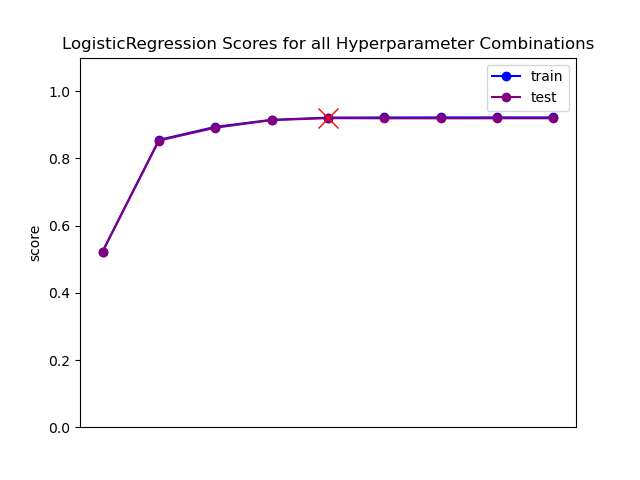
\includegraphics[width=\linewidth]{Latex_Report/report/Graphs/LR/scores_plot.png}
   \end{center}
        \vspace*{-5mm}
        \caption{\label{first_figure}}
\end{figure}

Next, we worked on the Random Forest classifier that fits a number of decision tree classifiers on various sub-samples of our dataset and uses averaging to improve the predictive accuracy while also controlling over-fitting to a satisfying degree. A hyper parameter search using GridSearchCV was conducted to find the best maximum depth and number of estimator values that provide us with the highest possible accuracy for our model. We then calculated the training and testing score values and determined the overfitting before generating a confusion matrix, a plot for the scores of each estimator and a plot displaying the feature importances for the top 25 words all shown in Figure~\ref{Second_figure} below. The model successfully achieved an accuracy of 91.11\%, a mean squared error of 8.89\% and a precision of 91.25\% with an overfitting value of 1.42.\\ 

\begin{figure}[h]
   \begin{center}
        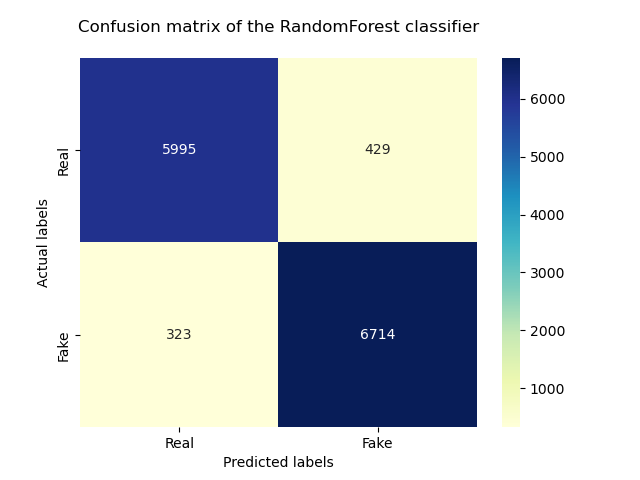
\includegraphics[width=\linewidth]{Latex_Report/report/Graphs/RF/confusion_matrix.png}
        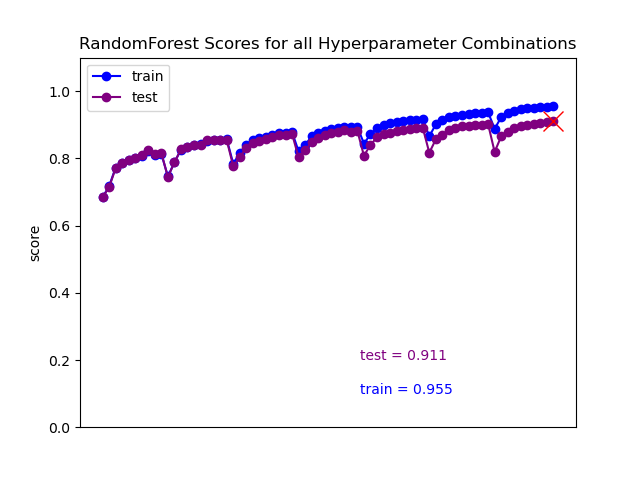
\includegraphics[width=\linewidth]{Latex_Report/report/Graphs/RF/scores_plot.png}
        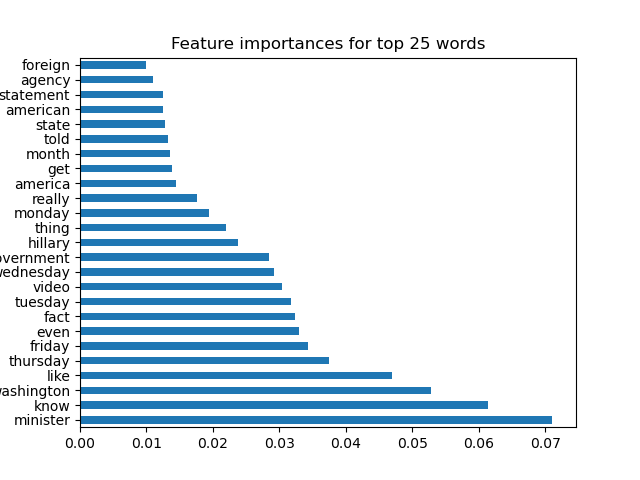
\includegraphics[width=\linewidth]{Latex_Report/report/Graphs/RF/feature_importances.png}
   \end{center}
        \vspace*{-5mm}
        \caption{\label{Second_figure}}
\end{figure}

Decision Tree classifier was the third model constructed with the goal of creating a classifier that predicts the correct label for a particular word by learning simple decision rules inferred from the training data features. A hyper parameter search using GridSearchCV and various max\_depth values was conducted to obtain the best accuracy possible and to help us in generating the training and testing accuracy scores. The model's overfitting value was also calculated and the best estimator was then used to generate the predictions and display the confusion matrix as well as the score graph shown in Figure~\ref{Third_figure} below. The model successfully achieved an accuracy of 86.14\%, a mean squared error of 13.86\% and a precision of 86.12\% with an overfitting value of 1.096.
 
\begin{figure}[h]
   \begin{center}
        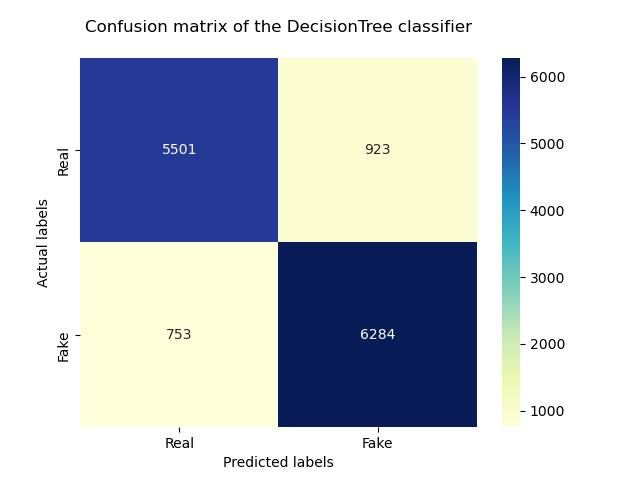
\includegraphics[width=\linewidth]{Latex_Report/report/Graphs/DT/confusion_matrix.png}
        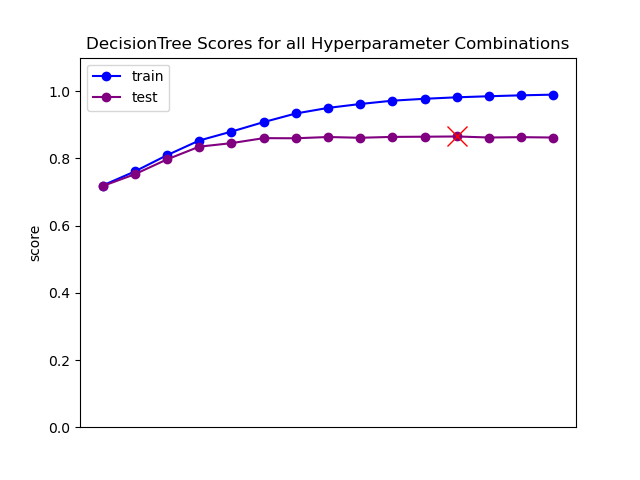
\includegraphics[width=\linewidth]{Latex_Report/report/Graphs/DT/scores_plot.png}
   \end{center}
        \vspace*{-8mm}
        \caption{\label{Third_figure}}
\end{figure}

Multinomial Naive Bayesian model was the next to be constructed given that it is suitable for classification of discrete features such as the tokenized text in our preprocessed dataset. We started by using GridSearchCV to perform a hyper parameter search that allowed us to choose the best accuracy to fit our data. We used the corresponding sklearn library to generate our model and then calculated the training and testing scores as well as the overfitting before we could plot our data. Next, we picked the best estimator we found and made the predictions, generated a confusion matrix and displayed a score graph as shown in Figure~\ref{fourth_figure}. The model successfully achieved an accuracy of 87.408\%, a mean squared error of 12.59\% and a precision of 90.01\% with an overfitting value of 0.022. 

\begin{figure}[h]
   \begin{center}
        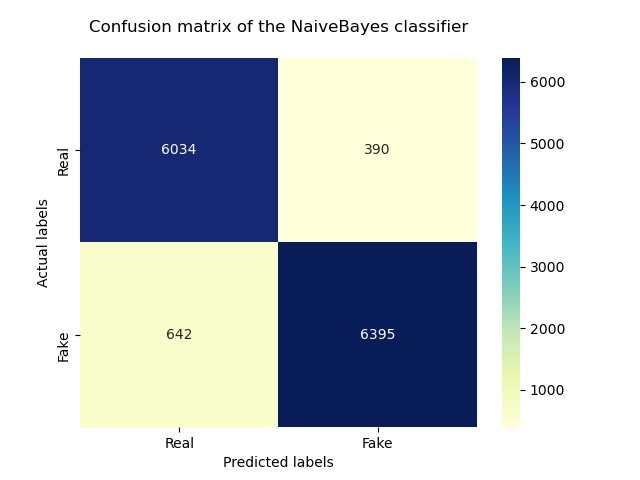
\includegraphics[width=\linewidth]{Latex_Report/report/Graphs/NB/confusion_matrix.png}
        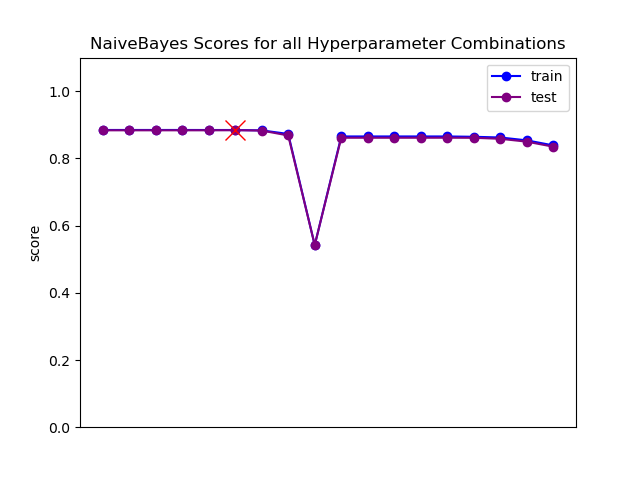
\includegraphics[width=\linewidth]{Latex_Report/report/Graphs/NB/scores_plot.png}
   \end{center}
        \vspace*{-8mm}
        \caption{\label{fourth_figure}}
\end{figure}

A Support Vector Machine model, which is a form of supervised learning, was then used to further help us in our quest for category prediction and classification. This model had an advantage of being memory efficient in the sense that it uses a subset of training points in the decision function called support vectors. In terms of the parameters used, we performed a hyper parameter search over 2 types of kernels, namely a Gaussian kernel of type 'rbf' and a linear kernel, as well as various values for C and gamma. This allowed us to obtain the best estimator to calculate the training and testing scores as well as to determine overfitting and perform prediction calculations. A plot for the scores of each estimator as well as a confusion matrix shown in Figure~\ref{fifth_figure} were generated to help us visualize our results. The model successfully achieved an accuracy of 60.73\%, a mean squared error of 39.27\% and a precision of 57.89\%.

\begin{figure}[h]
   \begin{center}
        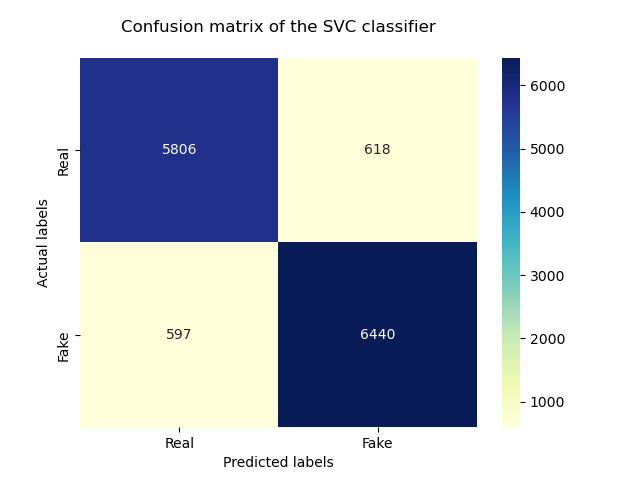
\includegraphics[width=\linewidth]{Latex_Report/report/Graphs/SVC/confusion_matrix.png}
        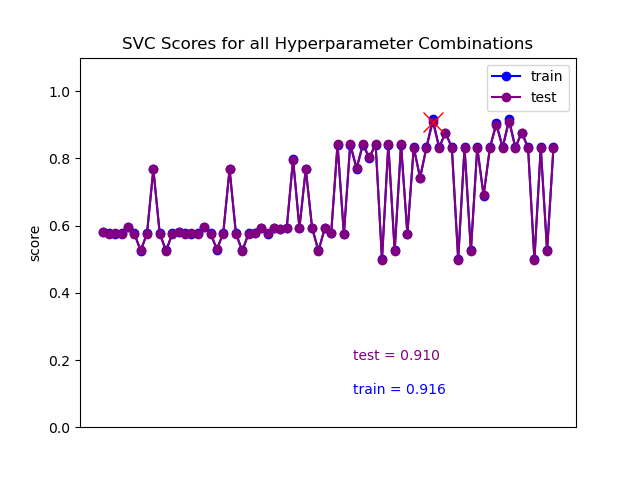
\includegraphics[width=\linewidth]{Latex_Report/report/Graphs/SVC/scores_plot.png}
   \end{center}
        \vspace*{-5mm}
        \caption{\label{fifth_figure}}
\end{figure}

Finally, a neural network was constructed 

%------------------------------------------------------------------------
\section{Conclusions}

\textcolor{blue}{Summarize what you could and could not conclude based on your experiments.
The ”References” section (bibliography) is optional. If you cite any books, websites, or academic papers, then you can add them to bibliography.bib and cite them in this re- port. Otherwise delete the references section.}

As discussed in the previous section our quest for article classification involved training various types of classifiers each taking their own set of parameters to achieve the most ideal results possible. We notice that logistic regression had the highest accuracy at 91.34\% when it came to correctly classifying our tokenized data into the Fake and Real categories. The confusion matrix generated for this model shows that it correctly classified 6014 words into the "Real" category and 6618 words into the "Fake" category and overfitting. The degree of overfitting for this classifier was also the lowest obtained at 0.009. This allows us to conclude that logistic regression classifier was the best model to use on our preprocessed data. 

Logistic regression was closely followed by the Random forest classifier with a classification accuracy of 91.11\%. The confusion matrix generated for this classifier shows very similar results to that of the logistic regression with 6060 words correctly classified into the "Real" category and 6675 words into the "Fake" category. The model, however, had a much higher overfitting value at 1.421. This means that although the classifiers were very close in terms of their accuracy, logistic regression remains at an advantage given that it had much less overfitting of data. 

The Multinomial Naive Bayesian model comes in third place in terms of performance with a classification accuracy of 87.41\%. Its confusion matrix shows that the model was able to successfully classify 6011 words into the "Real" category and 6206 words into the "Fake" category. The model has an advantage over the other two that it was the fastest to run and classify the data with a very low degree of overfitting at 0.022. In total the model took approximately 4 seconds to run from start to finish including the hyper parameter search that occupies the bulk of execution time. Perhaps this model would be a better fit to use compared to the logistic regression classifier if the goal is to achieve speed over accuracy. 

Decision Tree Classifier follows the Bayesian model closely with a classification accuracy of 86.14\%. Its confusion matrix shows that the mode was able to correctly classify 5674 words into the "Real" category and 6366 words into the "Fake" category. The model was significantly slower to run than the Bayesian model at 1.2 minutes vs the 3 seconds the Bayesian model took to classify our data. It also had a much higher overfitting value at 1.096 and thus we can conclude that the Naive Bayesian model is better employed to solve our particular problem on the provided dataset.  

Lastly the support vector machine classifier was the slowest to run out of all classifiers taking approximately 10.8 minutes to fully classify the data. It had the lowest classification accuracy of 60.73\% compared to other models and an overfitting value of 0.142. The model was successfully able to classify 1929 words into the "Real" category compared and 6559 into the "Fake" category. This information allows us to conclude that although the overfitting value for the model was relatively low, that advantage is outweighed by the slow run time for the model and a logistic regression model can achieve better results at a faster pace and with significantly less overfitting. 

Finally the CNN.... 

{\small
\raggedright
\bibliographystyle{ieeetr}
\bibliography{bibliography}
}

\newpage
\appendix


%-------------------------------------------------------------------------
\section*{Appendix: Extra Results (Optional)}

% DELETE THIS TEXT
\textcolor{blue}{If you want to include extra more detailed results that did not fit within the main report, include them here. Or, you can just delete this example section.}

multiple citations \cite{breiman2001statistical,bishop2006pattern}.

\begin{table*}[!hb]\centering
   \begin{center}
   \begin{tabular}{|l|c|c|c|c|c|}
   \hline
    Classifier & Accuracy & Mean Squared Error & Precision & Recall & fscore\\
   \hline\hline
   Naive Bayes & 92.33\% & 27.7\% & 94.25\% & 90.87\% & 92.53\% \\
   Decision Tree & 99.22\% & 8.79\% & 99.03\% & 99.48\% & 99.26\% \\
   Random forest & 94.40\% & 23.60\% & 93.99\% & 95.41\% & 94.69\%\\
   Support Vector Machine & 90.90\% & 30.04\% & 91.24\% & 91.51\% & 91.38\% \\
   Logistic Regression & 99.08\% & 9.55\% & 99.14\% & 99.10\% & 99.13\% \\
   Central Neural Network & 0.00\% & 0.00\% & 0.00\% & 0.00\% & 0.00\% \\
   \hline
   \end{tabular}
   \end{center}
   \caption{Summary of Model Results\label{first_table}}
\end{table*}

\end{document}
